%%%%%%%%%%%%%%%%%%%%%%%%%%%%%%%%%%%%%%%%%%%%%%%%%%%%%%%%%%%%%%%%%%%
%                                                                 %
%  GEANT manual in LaTeX form                                     %
%                                                                 %
%  Michel Goossens (for translation into LaTeX)                   %
%  Version 1.00                                                   %
%  Last Mod. Jan 24 1991  1300   MG + IB                          %
%                                                                 %
%%%%%%%%%%%%%%%%%%%%%%%%%%%%%%%%%%%%%%%%%%%%%%%%%%%%%%%%%%%%%%%%%%%
\Documentation{F.Bruyant}
\Submitted{01.10.84}      \Revised{10.03.94}
\Version{Geant 3.21}\Routid{GEOM001}
\Makehead{The geometry package}

The geometry package has two main functions:

\begin{enumerate}
\item define, during the initialisation of the program,
the geometry in which the particles will be tracked;
\item communicate, during the event processing phase, to the tracking 
routines the information for 
the transport of the particles in the geometry which has been defined.
\end{enumerate}

The present section reviews the concepts of the geometry package and explains
how the geometrical information should be provided by the user.
It is important to point out that, once the geometry has been defined,
the tracking of particles through the different volumes proceeds without any
intervention from the user {\tt [TRAK]}. 

The connection between the
geometry and tracking packages is established by the subroutines
\Rind{GMEDIA}/\Rind{GTMEDI}, \Rind{GTNEXT}/\Rind{GNEXT} and
\Rind{GINVOL} which answer respectively the questions:
\begin{itemize}
\item    In which volume is a given point ?
\item    What is the distance to the nearest volume along the trajectory
of the particle ?
\item    What is the distance to the nearest volume ?
\item    Is a given point still in the current volume ?
\end{itemize}
The routines \Rind{GTMEDI}, \Rind{GTNEXT} are used in a dynamic context,
at tracking time, when the
knowledge of the track direction can be used to save time.
\section{ The volume definition }

Experimental setups, as complex as the LEP\footnote{The Large Electron Positron
collider in operation at CERN.} detectors, can be described 
rather accurately through the definition of a set of {\it volumes}.
Each {\it volume} is given a {\it name} and is characterised by:
\begin{itemize}
\item a {\it shape} identifier, specifying one of the basic
          geometrical shapes available {\tt [GEOM050]};
\item   the {\it shape} parameters, giving the dimensions of the volume;
\item   a local reference system, with origin and axes defined
for the each shape;
\item    the physical properties, given by a set of constants describing the
homogeneous {\it material} which fills the volume ({\tt [CONS]});
\item  additional properties, known as {\it tracking medium} parameters,
which depend on the characteristics of the volume itself (the
material identifier is one of the constants) and on its geometrical and
physical environment (properties of the neighbouring volumes, magnetic field, 
etc.) {\tt [CONS, TRAK]};
\item  a set of attributes, in connection with the drawing package
and the detector response package {\tt [DRAW, HITS]}.
\end{itemize}
Until it is {\it positioned} in a given reference frame,
a volume is an entity which has no spatial relation with the other volumes.
By convention, a unique initial volume has to be defined first
which will contain
all the other volumes. The reference frame intrinsic
to this volume is considered to be the master reference frame.

There are sixteen basic shapes in {\tt GEANT}, which are described in
{\tt [GEOM050]}.

\section{Volumes with contents}
A {\it volume} can be declared to have contents and as such it becomes a 
{\it mother}
volume. The contents are {\it either} predefined volumes which are explicitly 
positioned inside the mother, {\it or} new volumes which are implicitly defined
by a division mechanism applied to the mother. Positioning a volume with given 
shape and dimensions inside a mother volume is obtained by specifying its 
translation and rotation with respect to the mother reference frame. The user 
should make sure that no volume extends beyond the boundaries of its mother.

When a volume is positioned, the user gives it a {\it number}. Multiple copies 
of the same volume can be positioned inside the same or different mothers
as long as their copy numbers differ.
The contents of the positioned volume are reproduced 
in all copies. 

Mother volumes can be divided by planes along the three axes ($ x, y, z$),
radially along $R_{xy}$, or along the spherical coordinates of a 
polar system: $R$, $\theta$ and $\phi$. The axis along which it is
possible to perform a division depend on the shape to be divided. The
general rule is that the result of the division be still a {\tt GEANT} shape.

A volume can be partially or totally divided.
The division process
generates a number of {\it cells}, which are considered as new volumes.
The cell dimensions are computed
according to the number of divisions or the step size. A cell, as any
other volume, can again be divided, or have other
volumes positioned into it. Any operation of positioning or division
performed on one cell is repeated to all the cells resulting
from the division. A volume can be {\it either} divided {\it or} have
contents, but not the two things together.

These operations define a physical tree with several
levels. The material and properties of the contents replace the
ones of the mother within the space region they occupy.
A {\tt volume} is therefore defined not only by its intrinsic characteristics
but also by those of its {\it descendants}, namely its contents (by
division or positioning), the contents of its contents, etc.

\section{ Overlapping volumes, see also {\tt [GEOM020]} }
The user may define volumes which have no relation with the real
objects. It is sometimes convenient to make use of such volumes,
to artificially delimit regions with simple shapes.
Doing this, it may happen that
volumes partially overlap each other. (A volume positioned inside a mother is
obviously not regarded as overlapping the mother).

It is possible in {\tt GEANT} to handle partially overlapping volumes, but
there are some implications that the user should be aware of.
A flag {\tt 'ONLY'/'MANY'} is assigned to each copy of a given volume at the 
moment this is positioned. The {\tt 'MANY'} option indicates that
a point found in this volume could also be in other volumes which are
not its direct descendants. If one of the
overlapping volumes where the point is found is declared as {\tt 'ONLY'}, the
geometry subroutines will give priority to this volume, 
and the search stops.
If a point is inside several {\tt 'MANY'} volumes and outside all {\tt 'ONLY'}
ones, priority will be given to the volume
found at the deepest level, or to the first found, if there are many
valid {\tt 'MANY'} candidates at the same level. In order to avoid ambiguities,
two overlapping {\tt 'MANY'} volumes should in general
have the same tracking medium.

\section{The physical tree}
An example of a 4 level physical tree with embedded volumes and
the corresponding geometrical configuration are shown in fig~\ref{fg:geom001-1}.

\begin{figure}[hbt]
      \centering
      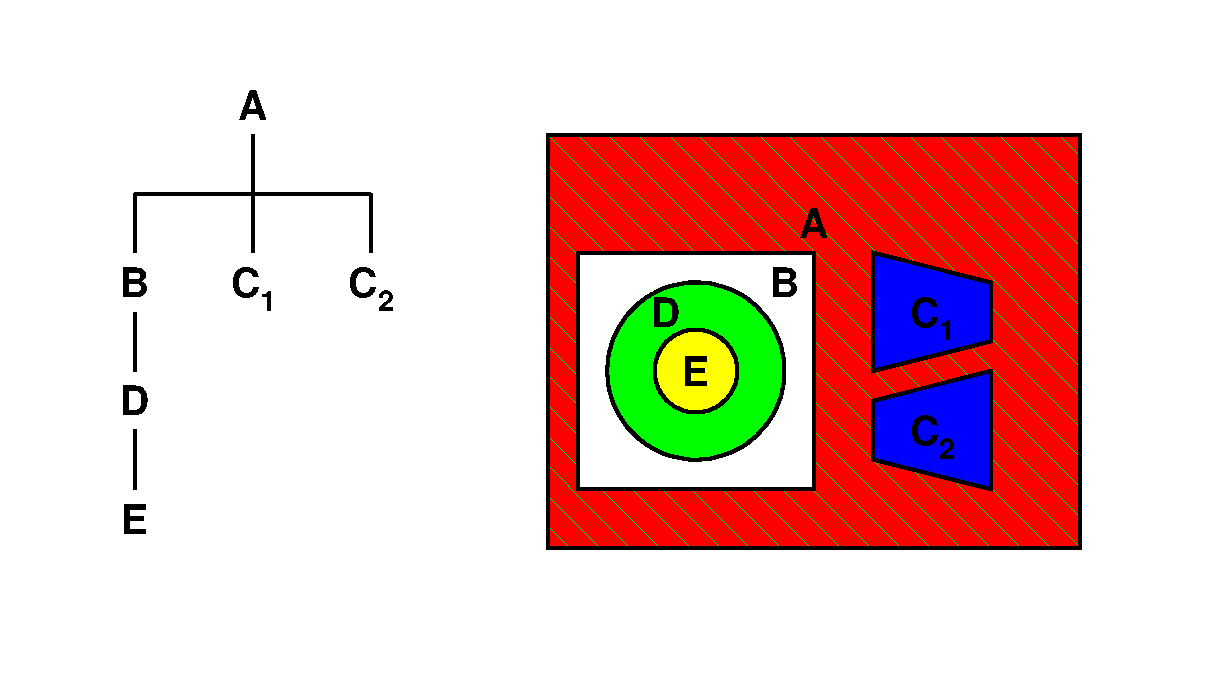
\epsfig{file=eps/geom001-1.eps,width=16cm}
      \caption{Example of geometrical tree structure}
      \label{fg:geom001-1}
\end{figure}

where A and B are {\tt BOX}es, C a {\tt TRAP}ezoid, and D and E {\tt TUBE}s
(see {\tt [GEOM050]} for more detail).
Notice that the same physical configuration could be described as well though
a 3 level tree if D were defined as a {\it hollow}
{\tt TUBE}, with inner radius non-zero and E
directly positioned into B.
The package accepts a maximum of 15 levels, which should be
enough to represent the fine details of a complex structure.
\section{The data structures {\tt JVOLUM} and {\tt JGPAR}
and the common {\tt /GCVOLU/}}

In practice, the physical tree is not represented as such in the
data part of the program. Instead, a logical tree structure is defined,
the {\tt JVOLUM} data structure, which describes the arrangement of
volumes in a compact and recurrent way. Each generic volume appears once,
and once only, and carries the information relevant to the volume itself
and to its contents, if any, by reference to the
generic volumes corresponding to those contents.
In the situation where division or multiple copies occur, there
is no longer a one-to-one correspondence between a volume in the
logical tree and a region in space. Information has to be added at
tracking time to identify which division cell or which copy was considered
at each depth level along the path through the physical tree. This
information is stored by the subroutine \Rind{GMEDIA}/\Rind{GTMEDI}, for the
current point of the current track, in the common \FCind{/GCVOLU/}. It includes
the current level number {\tt NLEVEL} and, for each level, starting from the
first mother volume, the identification of the corresponding volume, e.g.:
{\tt NAME}, {\tt NUMBER}, {\tt 'ONLY'/'MANY'} flag, translation and rotation
with respect to the master reference frame and so on. 
The number of shape parameters
and pointers to the vector describing the actual values of those
parameters, for each level, are stored in the data part and in the link
part, of the data structure {\tt JGPAR}, respectively.

\section{The user tools }

The geometry through which the particles are transported is defined by the
user via a set of calls to subroutines of the {\tt GEANT} package.

The user can define a volume through a call to the subroutine:
\begin{DLtt}{MMMMMMMM}
\item[\Rind{GSVOLU}] define ({\it instantiate}) a volume by giving a 
{\tt NAME} and the actual parameters to a shape; the position of the volume 
inside the bank {\tt JVOLUM} is returned. If any of the parameters which
express a length is negative, {\tt GEANT} will assign to this parameter
at tracking time
the maximum value allowed, without protruding out of the mother 
which contains the particle transported.

A shape can be instantiated
into a volume also without actual parameters. These will then be supplied
when positioning each copy of the volume via the \Rind{GSPOSP} routine (see
below). This allows to have many {\it similar} volumes with the same name
and shape, but different actual parameters in each copy.
\end{DLtt}

The user can position a volume through a call to either one of the following 
subroutines:

\begin{DLtt}{MMMMMMMM}
\item[\Rind{GSPOS}] position a copy of a volume inside its mother with respect 
to the mother's reference system. A a point in space, a rotation matrix
index, a copy number and the {\tt 'ONLY'/'MANY'} flag are supplied;
\item[\Rind{GSPOSP}] position a copy of a volume which has been instantiated
without actual parameters inside its mother with respect to the mother reference
system. The parameters of the copy being positioned are supplied as well.
The volumes will be identified by name and copy number as for multiple copies
of the same volume.
\end{DLtt}
The user can divide a volume through a call to either one of the following
subroutines:

\begin{DLtt}{MMMMMMM}
\item[\Rind{GSDVN}] divide a volume in a given {\it number} of cells completely
filling the mother. In this case the cell tracking medium
is assumed to be the same as for the mother. See also \Rind{GSDVN2}.
\item[\Rind{GSDVT}] divide a volume with slices of a given {\it step}.
The cell tracking medium can be different from the one of the mother.
See also \Rind{GSDVT2}.
\item[\Rind{GSDVX}] divide a volume starting from a given offset. In addition 
to {\tt STEP} and {\tt NDIV} (with at least one of them positive to be 
effectively useful), the origin of the first cell, the cell tracking medium 
and eventually the computed (maximum) number of divisions must be specified.
\end{DLtt}


\section{Geometrical information retrieval}

The parameters of a volume may depend on the physical tree which leads to
this volume. The dimensions of one of the slices of a cone divided along
{\tt Z} depends on which slice we consider. So a volume is completely
defined only if we specify the path in the tree. This is composed by the
name and copy number of the volumes containing the one we are interested
in, from the first mother.

Given this information, the routine \Rind{GLVOLU} is capable to fill the
common \FCind{/GCVOLU/}, and the structure {\tt JGPAR} with the actual
parameters of the instance chosen.
